\newcommand{\chainle}{\ensuremath{\mathrel{\sqsubseteq}}}
\newcommand{\chainlt}{\ensuremath{\mathrel{\sqsubset}}}
\newcommand{\chainnotlt}{\ensuremath{\mathrel{\nsqsubset}}}
\newcommand{\wehave}{.\;}
\newcommand{\suchthat}{.\;}
\newcommand{\app}{\ensuremath{\mathrel{\triangleright}}}
\newcommand{\length}[1]{\ensuremath{\mathrm{length} \; #1}}
\newcommand{\ifthen}[2]{\ensuremath{\mathrm{if} \quad #1 \quad \mathrm{then} \quad #2}}
\renewcommand{\iff}{\ensuremath{\qquad\mathrm{iff}\qquad}}
\newcommand{\candidates}[2]{\ensuremath{\mathsf{candidates}_#1(#2)}}
\newcommand{\blockNo}[1]{\ensuremath{\mathtt{blockNo}(#1)}}
\newcommand{\selectviewle}{\ensuremath{\precsim}}

\chapter{Chain Selection}
\label{chainsel}

Chain selection is one of the central responsibilities of the chain database
(\cref{chaindb}). It of course depends on chain selection as it is defined  by
the consensus protocol (\cref{consensus:class:chainsel}), but needs to  take
care of a lot of operational concerns. In this chapter we will take a closer
look at the implementation of chain selection in the chain database, and state
some properties and sketch some proofs to motivate it.

\section{Comparing anchored fragments}
\label{chainsel:fragments}

\subsection{Introduction}

Recall from \cref{consensus:overview:chainsel} that while in the literature
chain selection is defined in terms of comparisons between entire chains, we
instead opted to model it in terms of a comparison between the \emph{headers} at
the tip of those chains (or rather, a \emph{view} on those headers defined by
the specific consensus protocol).

We saw in \cref{storage:inmemory} (specifically, \cref{storage:fragments}) that
the consensus layer stores chain fragments in memory (the most recent headers on
a chain), both for the node's own current chain as well as for upstream nodes
(which we refer to as ``candidate chains''). Defining chain selection in terms
of fragments is straight-forward when those fragments are non-empty: we simply
take the most recent header, extract the view required by the consensus protocol
(\cref{BlockSupportsProtocol}), and then use the consensus protocol's chain
selection interface to compare them. The question is, however, how to compare
two fragments when one (or both) of them is \emph{empty}. This problem is more
subtle than it might seem at first sight, and requires careful consideration.

We mentioned in \cref{consensus:overview:chainsel} that consensus imposes a
fundamental assumption that the strict extension of a chain is always (strictly)
preferred over that chain (\cref{prefer-extension}), and that consequently we
\emph{always} prefer a non-empty chain over an empty one (and conversely we
\emph{never} prefer an empty chain over a non-empty one). However, chain
fragments are mere proxies for their chains, and the fragment might be empty
even if the chain is not. This means that in principle it's possible we do not
prefer a non-empty fragment over an empty one, or indeed prefer an empty
fragment over a non-empty one. However, when a fragment is empty, we cannot rely
on the consensus protocol's chain selection because we have no header to give
it.

Let's consider under which conditions these fragments might be empty:

\begin{description}
\item[Our fragment]
Our own fragment is a path through the volatile database, anchored at the tip of
the immutable database (\cref{storage:fragments}). Under normal circumstances,
it will be empty only if our \emph{chain} is empty; we will refer to such empty
fragments as \emph{genuinely empty}.\footnote{We can distinguish between an empty
fragment of a non-empty chain and a (necessarily) empty fragment of an empty
chain by looking at the anchor point: if it is the genesis point, the chain must
be empty.} However, our fragment can also be empty even when our chain is not,
if due to data loss the volatile database is empty (or contains no blocks that
fit onto the tip of the immutable database).

\item[Candidate fragment]
A \emph{genuinely} empty candidate fragment, representing an empty candidate
chain, is never preferred over our chain. Unfortunately, however, the candidate
fragment as maintained by the chain sync client (\cref{chainsyncclient}) can
essentially be empty at any point due to the way that a switch-to-fork is
implemented in terms of rollback followed by roll forward: after a maximum
rollback (and before the roll forward), the candidate fragment is empty.
\end{description}

\subsection{Precondition}
\label{chainsel:fragments:precondition}

Since neither of these circumstances can be avoided, we must therefore impose a
precondition for chain selection between chain fragments to be definable:

\begin{definition}[Precondition for comparing chain fragments]
The two fragments must either both be non-empty, or they must intersect.
\end{definition}

In this chapter, we establish this precondition in two different ways:

\begin{enumerate}
\item When we construct candidates chains (potential chains that we may wish
to replace our own chain with), those candidate chains must intersect with
our own chain within $k$ blocks from its tip; after all, if that is not the
case, we would induce a roll back of more than $k$ blocks
(\cref{consensus:overview:k}).

\item When we compare fragments to each other, we only compare fragments from a
set of fragments that are all anchored at the same point (i.e., the anchor of
all fragments in the set is the same, though it might be different from the
anchor of our current fragment). Since they are all anchored at the same point,
they trivially all intersect with each other.
\end{enumerate}

There is one more use of fragment selection, which is rather more subtle;
we will come back to this in \cref{chainsyncclient:plausiblecandidates}.

\todo{TODO} TODO: Throughout we are talking about \emph{anchored} fragments
here. We should make sure that we discuss those somewhere.

\subsection{Definition}
\label{chainsel:fragments:definition}

We will now show that this precondition suffices to compare two fragments,
whether or not they are empty; we'll consider each case in turn.

\begin{description}

\item[Both fragments empty]
Since the two fragments must intersect, that intersection point can only
be the two anchor points, which must therefore be equal. This means that
two fragments represent the same chain: neither fragment is preferred
over the other.

\item[First fragment non-empty, second fragment empty]
Since the two fragments must intersect, that intersection can only be the
anchor of the second fragment, which can lie anywhere on the first fragment.

\begin{itemize}
\item If it lies at the \emph{tip} of the first fragment, the two fragments represent the
same chain, and neither is preferred over the other.
\item If it lies \emph{before} the tip of first fragment, the first fragment is
a strict extension of the second, and is therefore is preferred over the
second.
\end{itemize}

\item[First fragment empty, second fragment non-empty]
This case is entirely symmetric to the previous; if the intersection is the
tip of the second fragment, the fragments represent the same chain. Otherwise,
the second fragment is a strict extension of the first, and is therefore
preferred.

\item[Both fragments non-empty]
In this case, we can simply use the consensus protocol chain selection API
to compare the two most recent headers on both fragments.

\end{description}

Note that this relies critically on the ``prefer extension'' rule
(\cref{prefer-extension}).

\section{Preliminaries}
\label{chainsel:spec}

Recall from \cref{storage:components} that the immutable database stores a
linear chain, terminating in the \emph{tip} $I$ of the immutable database. The
volatile database stores a (possibly fragmented) tree of extensions to that
chain:
%
\begin{center}
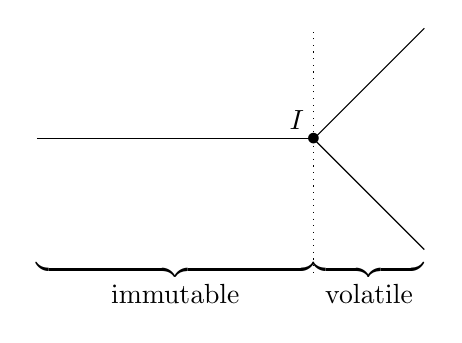
\begin{tikzpicture}
\draw (0,0) -- (100pt, 0) coordinate (immtip) node{$\bullet$} node[above left] {$I$};
\draw (immtip) -- ++(40pt,  40pt);
\draw (immtip) -- ++(40pt, -40pt);
\draw [dotted] (immtip) -- ++(0, 40pt);
\draw [dotted] (immtip) -- ++(0, -50pt);
\node at (50pt, -40pt) [below] {$\underbrace{\hspace{100pt}}_\textrm{immutable}$};
\node at (120pt, -40pt) [below] {$\underbrace{\hspace{40pt}}_\textrm{volatile}$};
\end{tikzpicture}
\end{center}
%
The node's \emph{current chain} is stored in memory as a chain fragment through
the volatile database, anchored at $I$.  When we start up the node, the chain
database must find the best possible path through the volatile database and
adopt that as our current fragment; every time a new block is added to the
volatile database, we have to recompute the new best possible path. In other
words, we maintain the following invariant:

\begin{definition}[Current chain invariant]
\label{current-chain-invariant}
The current chain is the best possible path through the volatile DB.
\end{definition}

``Best'' of course is according to the chain selection rule defined by the
consensus protocol (\cref{consensus:class:chainsel}). In this section we
describe how the chain database establishes and preserves this invariant.

\subsection{Notation}

So far we have been relatively informal in our description of chain selection,
but in order to precisely describe the algorithm and state some of its
properties, we have to introduce some notation.

\begin{definition}[Chain selection]
We will model chain selection as a transitive binary relation (\chainlt) between
valid chains (it is undefined for invalid chains), and let $C \chainle C'$ if
and only if $C \chainlt C'$ or $C = C'$. It follows that (\chainle) is a partial
order (reflexive, antisymmetric, and transitive).
\end{definition}

For example, the simple ``prefer longest chain'' chain selection rule could be
given as
%
\begin{equation*}
\tag{longest chain rule}
C \chainlt C'  \iff  \length{C} < \length{C'}
\end{equation*}

In general of course the exact rule depends on the choice of consensus protocol.
\Cref{prefer-extension} (\cref{consensus:overview:chainsel}) can now be
rephrased as
%
\begin{equation}
\label{eq:prefer-extension}
\forall C, B \wehave C \chainlt (C \app B)
\end{equation}

We will not be comparing whole chains, but rather chain fragments
(we will leave the anchor of fragments implicit):
%
\begin{definition}[Fragment selection]
We lift $\chainlt$ to chain fragments in the manner described in
\cref{chainsel:fragments}; this means that $\chainlt$ is undefined for two
fragments if they do not intersect (\cref{chainsel:fragments:precondition}).
\end{definition}

We also lift $\chainle$ to \emph{sets} of fragments, intuitively indicating that
a particular fragment is the ``best choice'' out of a set $\mathcal{S}$ of
candidate fragments:
%
\begin{definition}[Optimal candidate]
\begin{equation*}
\mathcal{S} \chainle F  \iff   \nexists F' \in \mathcal{S} \suchthat F \chainlt F'
\end{equation*}
(in other words, if additionally $F \in \mathcal{S}$, then $F$ is a maximal
element of $C$). This inherits all the preconditions of $\chainle$ on chains and
fragments.
\end{definition}

Finally, we will introduce some notation for \emph{computing} candidate
fragments:\footnote{In order to compute these candidates efficiently, the
volatile database must support a ``forward chain index'', able to efficiently
answer the question ``which blocks succeed this one?''.}

\begin{definition}[Construct set of candidates]
Given some set of blocks $V$, and some anchor $A$ (with $A$ either a block or
the genesis point), $$\candidates{A}{V}$$ is the set of chain fragments
anchored at $A$ using blocks picked from $V$.
\end{definition}

By construction all fragments in $\candidates{A}{V}$ have the same anchor, and
hence all intersect (at $A$); this will be important for the use of the
$\chainle$ operator.

\subsection{Properties}

In the following we will use ($F \app B$) to denote appending block $B$ to chain
$F$, and lift this notation to sets, so that for some set of blocks
$\mathcal{B}$ we have
%
\begin{equation*}
F \app \mathcal{B} = \{ F \app B \mid B \in \mathcal{B} \}
\end{equation*}

\begin{lemma}[Properties of the set of candidates]
\label{candidates:properties}
The set of candidates computed by $\candidates{A}{V}$ has the following
properties.

\begin{enumerate}

\item \label{candidates:prefixclosed}
It is prefix closed:
\begin{equation*}
\forall F, B \wehave
\ifthen
  {(F \app B) \in \candidates{A}{V}}
  {F \in \candidates{A}{V}}
\end{equation*}

\item \label{candidates:appendnew}
If we add a new block into the set, we can append that block to existing
candidates (where it fits):
\begin{equation*}
\ifthen
  {F \in \candidates{A}{V}}
  {F \app B \in \candidates{A}{V \cup \{ B \}}}
\end{equation*}
provided $F$ can be extended with $B$.

\item \label{candidates:monotone}
Adding blocks doesn't remove any candidates:
\begin{equation*}
\candidates{A}{V} \subseteq \candidates{A}{V \cup \{B\}}
\end{equation*}

\item \label{candidates:musthavenew}
If we add a new block, then any new candidates must involve that new block:
\begin{equation*}
\ifthen
  {F \in \candidates{A}{V \cup \{B\}}}
  {F \in \candidates{A}{V} \text{ or } F = (\ldots \app B \app \ldots)}
\end{equation*}

\end{enumerate}
\end{lemma}

The next lemma says that if we have previously found some optimal candidate $F$,
and subsequently learn of a new block $B$ (where $B$ is a direct or indirect
extension of $F$), it suffices to find a locally optimal candidate \emph{amongst
the candidates that involve $B$}; this new candidate will also be a globally
optimal candidate.

\begin{lemma}[Focus on new block]
\label{focusonnewblock}
Suppose we have $F, F_\mathit{new}$ such that
\begin{enumerate}
\item \label{focusonnewblock:previouslyoptimal}
$\candidates{A}{V} \chainle F$
\item \label{focusonnewblock:optimalamongstnew}
$(\candidates{A}{V \cup \{B\}} \setminus \candidates{A}{V}) \chainle F_\mathit{new}$
\item \label{focusonnewblock:betterthanold}
$F \chainle F_\mathit{new}$
\end{enumerate}
Then
\begin{equation*}
\candidates{A}{V \cup \{B\}} \chainle F_\mathit{new}
\end{equation*}
\end{lemma}

\begin{proof}
Suppose there exists $F' \in \candidates{A}{V \cup \{B\}}$ such that
$F_\mathit{new} \chainlt F'$. By transitivity and
assumption~\ref{focusonnewblock:betterthanold}, $F \chainlt F'$. As
shown in \cref{candidates:properties} (\cref{candidates:musthavenew}), there are two possibilities:

\begin{itemize}
\item $F' \in \candidates{A}{V}$, which would violate
assumption~\cref{focusonnewblock:previouslyoptimal}, or
\item $F'$ must contain block $B$, which would violate
assumption~\cref{focusonnewblock:optimalamongstnew}.
\end{itemize}
\end{proof}

\section{Initialisation}
\label{chainsel:init}

The initialisation of the chain database proceeds as follows.

\begin{enumerate}

\item
\label{chaindb:init:imm}
Initialise the immutable database, determine its tip $I$, and ask the ledger DB
for the corresponding ledger state $L$ (see
\cref{ledgerdb:on-disk:initialisation}).

\item Compute the set of candidates anchored at the immutable database's tip
\label{chaindb:init:compute}
$I$ using blocks from the volatile database $V$
$$\candidates{I}{V}$$
ignoring known-to-be-invalid blocks (if any; see \cref{chaindb:invalidblocks})
and order them using $(\chainlt)$  so that we process better candidates
first.\footnote{Technically speaking we should \emph{first} validate all
candidates, and only then apply selection to the valid chains. We perform chain
selection first, because that is much cheaper. Both approaches are semantically
equivalent, since \lstinline!sortBy f . filter p = filter p . sortBy f! due to
the stability of \lstinline!sortBy!.} Candidates that are strict prefixes of
other candidates can be ignored (as justified by the ``prefer extension''
assumption, \cref{prefer-extension});\footnote{The implementation does not
compute candidates, but rather ``maximal'' candidates, which do not include such
prefixes.} we may reconsider some of these prefixes if we subsequently discover
invalid blocks (see \cref{chaindb:init:select}).

\item
\label{chaindb:init:select}
Not all of these candidates may be valid, because the volatile database stores
blocks whose \emph{headers} have been validated, but whose \emph{bodies} are
still unverified (other than to check that they correspond to their headers).
We therefore validate each candidate chain fragment, starting with $L$ (the
ledger state at the tip of the immutable database) each time.\footnote{We make
no attempt to share ledger states between candidates, even if they share a
common prefix, trading runtime performance for lower memory pressure.}

As soon as we find a candidate that is valid, we adopt it as our current chain.
If we find a candidate that is \emph{invalid}, we mark the invalid
block\footnote{There is no need to mark any successors of invalid blocks; see
\cref{chaindb:dont-mark-invalid-successors}.} (unless it is invalid due to
potential clock skew, see \cref{chainsel:infuture}), and go back to
step~\ref{chaindb:init:compute}. It is important to recompute the set of
candidates after marking some blocks as invalid because those blocks may also
exist in other candidates and we do not know how the valid prefixes of those
candidates should now be ordered.

\end{enumerate}

\section{Adding new blocks}
\label{chainsel:addblock}

When a new block $B$ is added to the chain database, we need to add it to the
volatile DB and recompute our current chain. We distinguish between the
following different cases.

Before we process the new block, we first run chain selection on any blocks that
had previously been temporarily shelved because their slot number was (just)
ahead of the wallclock (\cref{chainsel:infuture}). We do this independent of what
we do with the new block.\footnote{In a way, calls to \lstinline!addBlock! are
how the chain database sees time advance. It does not rely on slot length to do
so, because slot length is ledger state dependent.}

The implementation \lstinline!addBlock! additionally provides  client code with
various notifications throughout the process  (``block added'', ``chain
selection run'', etc.). We will not describe these notifications here.

\subsection{Ignore}

We can just ignore the block if any of the following is true.

\begin{itemize}

\item
The block is already in the immutable DB, \emph{or} it belongs to a branch which
forks more than $k$ blocks away from our tip, i.e.\footnote{The check is a
little more complicated in the presence of EBBs (\cref{ebbs}). This is relevant
if we switch to an alternative fork after a maximum rollback, and that
alternative fork starts with an EBB. It is also relevant when due to data
corruption the volatile database is empty and the first block we add when we
continue to sync the chain happens to be an EBB.}
%
\begin{equation*}
\blockNo{B} \leq \blockNo{I}
\end{equation*}
%
We could distinguish between between the block being on our chain or on a
distant fork by doing a single query on the immutable database, but it does not
matter: either way we do not care about this block.

We don't expect the chain sync client to feed us such blocks under normal
circumstances, though it's not impossible: by the time a block is downloaded
it's conceivable, albeit unlikely, that that block is now older than $k$.

\item
The block was already in the volatile database, i.e.
%
\begin{equation*}
B \in V
\end{equation*}

\item
The block is known to be invalid (\cref{chaindb:invalidblocks}).

\end{itemize}

\subsection{Add to current chain}
\label{chainsel:addtochain}

If $B$ fits onto the end of our current fragment $F$ (and hence onto our current chain) $F$, i.e.
%
\begin{itemize}
\item $F$ is empty, and $B_\mathit{pred} = I$
(where $I$ must necessarily also be the anchor of the fragment), or
\item $\exists F' \suchthat F = F' \app B_\mathit{pred}$
\end{itemize}
%
then any new candidates must be equal to or an extension of $F \app B$
(\cref{candidates:properties}, \cref{candidates:musthavenew}); this set is
computed by
%
\begin{equation*}
(F \app B \app \candidates{B}{V \cup \{B\}})
\end{equation*}
%
Since all candidates would be strictly preferred over $F$ (since they are
extensions of $F$), by \cref{focusonnewblock} it suffices to pick the best
candidate amongst these extensions. Apart from the starting point, chain
selection then proceeds in the same way as when we are initialising the database
(\cref{chainsel:init}).

This case takes care of the common case where we just add a block to our chain,
as well as the case where we stay with the same branch but receive some blocks
out of order. Moreover, we can use the \emph{current} ledger state as the
starting point for validation.

\subsection{Store, but don't change current chain}

When we are missing one of the (transitive) predecessors of the block, we store
the block but do nothing else. We can check this by following back pointers
until we reach a block $B'$ such that $B' \notin V$ and $B' \neq I$. The cost of
this is bounded by the length of the longest fragment in the volatile DB, and
will typically be low; moreover, the chain fragment we are constructing this way
will be used in the switch-to-fork case
(\cref{chainsel:switchtofork}).\footnote{The function that constructs these
fragments is called \lstinline!isReachable!.}

At this point we \emph{could} do a single query on the immutable DB to check if
$B'$ is in the immutable DB or not. If it is, then this block is on a distant
branch that we will never switch to, and so we can ignore it. If it is not, we
may or may not need this block later and we must store it; if it turns out we
will never need it, it will eventually be garbage collected (\cref{chaindb:gc}).

An alternative and easier approach is to omit the check on the immutable DB,
simply assuming we might need the block, and rely on garbage collection to
eventually remove it if we don't. This is the approach we currently use.

\subsection{Switch to a fork}
\label{chainsel:switchtofork}

If none of the cases above apply, we have a block $B$ such that

\begin{enumerate}
\item \label{chainsel:switchtofork:notinvoldb}
$B \notin V$
\item \label{chainsel:switchtofork:notinimmdb}
$\blockNo{B} > \blockNo{I}$ (and hence $B$ cannot be in the immutable DB)
\item \label{chainsel:switchtofork:connected}
For all transitive predecessors $B'$ of $B$ we have $B' \in V$ or $B' = I$.
In other words, we must have a fragment
$$F_\mathit{prefix} = I \app \ldots \app B$$
in $\candidates{I}{V \cup \{B\}}$.
\item \label{chainsel:switchtofork:doesnotfit}
(Either $F$ is empty and $B_\mathit{pred} \neq I$, or) $\exists F', B' \suchthat
F = F' \app B'$ where $B' \neq B_\mathit{pred}$; i.e., block does not fit onto
current chain.\footnote{\Cref{chainsel:switchtofork:connected} rules out the
first option: if $B_\mathit{pred} \neq I$ then we must have $B_\mathit{pred} \in
V$ and moreover this must form some kind of chain back to $I$; this means that
the preferred candidate cannot be empty.}
\end{enumerate}

We proceed in similar fashion to the case when the block fit onto the tip of our
chain (\cref{chainsel:addtochain}). The new candidates in $\candidates{I}{V \cup
\{B\}}$ must involve $B$ (\cref{candidates:properties},
\cref{candidates:musthavenew}), which in this case means they must all be
extensions of $F_\mathit{prefix}$; we can compute these candidates
using\footnote{The implementation of the chain database actually does not
construct fragments that go back to $I$, but rather to the intersection point
with the current chain. This can be considered to be an optimisation of what we
describe here.}
$$I \app \ldots \app B \app \candidates{B}{V \cup \{B\}}$$
Not all of these fragments might be preferred over the current chain; we filter
those out.\footnote{Recall that the current chain gets special treatment: when
two candidates are equally preferable, we can pick either one, but when a
candidate and the current chain are equally preferable, we must stick with the
current chain.} We then proceed as usual, considering each of the remaining
fragments in $(\chainle)$ order, and appeal to \cref{focusonnewblock}
again to conclude that the fragment we find in this way will be an optimal
candidate across the entire volatile database.


%
% *
%
% *
%
%
% It is worth pointing out that we do _not_ rely on `F_prefix` being longer than
% the current chain. Indeed, it may not be: if two leaders are selected for the
% same slot, and we _receive_ a block for the current slot before we can _produce_
% one, our current chain will contain the block from the other leader; when we
% then produce our own block, we end up in the switch-to-fork case; here it is
% important that `preferCandidate` would prefer a candidate chain (the chain that
% contains our own block) over our current chain, even if they are of the same
% length, if the candidate ends in a block that we produced (and the current chain
% does not); however, the `ChainDB` itself does not need to worry about this
% special case.
%
% [let's be explicit about the difference between current chain and self
% produced blocks]
%

\section{In-future check}
\label{chainsel:infuture}

As we saw in \cref{chainsel:spec}, the chain DB performs full
block validation during chain selection. When we have validated a block, we then
do one additional check, and verify that the block's slot number is not ahead of
the wallclock time (for a detailed discussion of why we require the block's
ledger state for this, see \cref{time}, especially
\cref{time:block-infuture-check}). If the block is far ahead of the wallclock,
we treat this as any other validation error and mark the block as invalid.

Marking a block as invalid will cause the network layer to disconnect from the
peer that provided the block to us, since non-malicious (and non-faulty) peers
should never send invalid blocks to us. It is however possible that an upstream
peer's clock is not perfectly aligned with us, and so they might produce a block
which \emph{we} think is ahead of the wallclock but \emph{they} do not. To avoid
regarding such peers as malicious, the chain database supports a configurable
\emph{permissible clock skew}: blocks that are ahead of the wallclock by an
amount less than this permissible clock skew are not marked as invalid, but
neither will chain selection adopt them; instead, they simply remain in the
volatile database available for the next chain selection.

It is constructive to consider what happens if \emph{our} clock is off, in
particular, when it is slow. In this scenario \emph{every} (or almost every)
block that the node receives will be considered to be in the future. Suppose we
receive two consecutive blocks $A$ and $B$. When we receive $A$, chain selection
runs, we find that $A$ is ahead of the clock but within the permissible clock
skew, and we don't adopt it. When we then receive $B$, chain selection runs
again, we now discover the $A, B$ extension to our current chain; during
validation we cut off this chain at $B$ because it is ahead of the clock, but we
adopt $A$ because it is now valid.  In other words, we are always behind one
block, adopting each block only when we receive the \emph{next} block.

\begin{bug}
One problem with this scheme is that if we receive a block $B$ which is ahead of
the clock when we receive it, we might never notice it if block $B$ is not (yet)
connected to our chain: by the time we receive the missing blocks (which connect
$B$ to our chain), $B$ might no longer be ahead of the clock and we might adopt
it, even if $B$ was ahead by more than the permissible clock skew.

We could avoid this problem if we stored the time we received a block alongside
the block in the volatile database, but in the current design, the volatile
database does not store \emph{any} information on disk apart from raw blocks,
so this would be quite a significant design change.
\end{bug}

\section{Sorting}

In this chapter we have modelled chain selection as a partial order
$(\chainle)$. This suffices for the formal treatment, and in theory also
suffices for the implementation. However, at various points during the chain
selection process we need to \emph{sort} candidates in order of preference. We
can of course sort values based on a preorder only (topological sorting), but we
can do slightly better. Recall from \cref{consensus:class:chainsel} that we
require that the \lstinline!SelectView! on headers must be a total order. We can
therefore define

\begin{definition}[Same select view]
Let $C \selectviewle C'$ if the select view at the tip of $C$ is less than
or equal to the select view at the tip of $C'$.
\end{definition}

(\selectviewle) forms a total preorder (though not a partial order); if $C
\selectviewle C'$ \emph{and} $C' \selectviewle C$ then the select views at the
tips of $C$ and $C'$ are equal (though they might be different chains, of
course). Since $C \selectviewle C'$ implies $C' \chainnotlt C$, we can use this
preorder  to sort candidates (in order words, we will sort them \emph{on} their
select view, in Haskell-parlance).
